
\documentclass[12pt]{article}  
%The article class is a very basic type of document for writing
\usepackage[margin=1in]{geometry}  %Adjust margins, formatting

\usepackage{amsmath}  
\usepackage{amssymb}  
\usepackage{amsfonts}  
%These packages add commands for useful symbols and fonts and things like that.
%Most of the time, these are all you need.

\usepackage{textcomp, gensymb}  %Gives more symbols, like /degree

\usepackage{amsthm}
\usepackage{adjustbox}
\usepackage{graphicx}

\usepackage{fancyhdr}  %Header and Footer formatting
%\pagestyle{fancy}  
%\renewcommand{\headrulewidth}{0.4pt}
\renewcommand{\footrulewidth}{0.4pt}
\setlength{\headheight}{15pt}

%Header and Footer Information
\lhead{}  %Replace with your name
\chead{}
\rhead{}  %Replace "Title" with the name of the assignment
\cfoot{\thepage\ of \ref{NumPages}}  %Counts the pages.

\makeatletter        %This provides a total page count as \ref{NumPages}
\AtEndDocument{\immediate\write\@auxout{\string\newlabel{NumPages}{{\thepage}}}}
\makeatother

\usepackage{amsthm}  %This will create the Problem environment

\usepackage[nottoc]{tocbibind} % for table of contents
\usepackage{multicol}
\usepackage{listings}
\usepackage{pgfplots}
\usepackage[section]{placeins}

\setlength{\headheight}{18pt} 

\title{A History of Cryptography and Cryptanalysis}
\date{\today}
\author{Christopher Colahan\\ Simpson College}

\begin{document}
%title page
\maketitle
\newpage

%table of contents page
\tableofcontents
\listoffigures
\newpage


%main content

%abstract area
\section{Abstract}
Cryptography is used every day to secure private information. Since the invention of the first ciphers
millennia ago, ciphers have been continuously created and broken. The history of cryptography and
cryptanalysis is examined, starting with the transposition and monoalphabetic substitution ciphers of the
ancient Greeks and Romans. Next, frequency analysis is examined as a technique to break monoalphabetic
and polyalphabetic substitution ciphers and an example implementation is provided. Finally, modern cryptography and various cryptanalysis techniques are examined.

\section{Antiquated Cryptography}
\subsection{Transposition Ciphers}
A transposition cipher rearranges the order of the plaintext to create the ciphertext. Two common transposition ciphers are the rail fence and columnar ciphers. In a columnar cipher, the plaintext is written horizontally with a fixed number of characters on each row. The cipher text is obtained by reading each column of the grid \cite{appcrypt}. Transposition ciphers are commonly added to other ciphers to make them more secure.

A technique to determine if a ciphertext is the result of a transposition cipher is to analyze the ciphertext with frequency analysis. If the frequency analysis is performed on the ciphertext and the result is close to the frequency of normal English text, then the cipher is likely to be a transposition cipher \cite{appcrypt}.

\subsection{Monoalphabetic Substitution Ciphers}

A monoalphabetic substitution cipher uses a mapping from one alphabet to another. For convenience converting between the English alphabet and $\mathbb{Z}_{26}$, a mapping $M$: $\{A,B,..., Z\} \rightarrow \mathbb{Z}_{26}$ is defined where $A\mapsto 0$, $B\mapsto 1$, ... $Z\mapsto 25$. Then $M^{-1}$ is defined to be $0\mapsto A$, $1\mapsto B$, ... $25\mapsto Z$.

\subsubsection{Shift Ciphers}
Shift ciphers work by shifting the symbols in the plaintext by an amount. For example, if we are using the English alphabet, then there are $n=26$ possible symbols. We could then choose some $k$, $0<k<n$ for our key. In our notation, this would look like
$$E(p_i,k)=M^{-1}(M(p_i)+k\text{ (mod $n$)}).$$
To get the deciphering function, we shift backwards:
$$D(c_i,k)=M^{-1}(M(c_i)-k\text{ (mod $n$)}).$$

\cite[pg. 98]{absalg}

\subsubsection{Homophonic Substitution Ciphers}
A homophonic substitution cipher is a substitution cipher that maps each symbol to one of more symbols in order to prevent frequency analysis from being used. 

For example, suppose we have 100 symbols $S=\{s_1,s_2,...s_{100}\}$. The letter $e$ would map to approximately 12 or those symbols, but the letter $a$ would only map to about 8 of those symbols.

Before enciphering, each letter is replaced at random with one of the symbols it maps to. This means that each symbol in the ciphertext only appears with a frequency of about 1\% \cite[pg. 53]{codebook}.

Homophonic substitution ciphers can be broken by using the occurrences of various character combinations. For example, $q$ is a rare character so is would be represented by only one symbol. Additionally, $u$ is represented by three symbols. Since $q$ is always followed by $u$, if a symbol in the ciphertext is always followed by one of three symbols, the characters probably represent $q$ and $u$ \cite[pg. 54]{codebook}. Similar techniques can be used to determine the rest of the symbols.

\subsection{Polyalphabetic Substitution Ciphers}
A polyalphabetic substitution cipher uses multiple monoalphabetic substitution ciphers to generate more possibilities for the ciphertext.

\subsubsection{Vigen\`{e}re Cipher}
The vigen\`{e}re cipher uses 26 alphabets to encrypt plaintext. A key is also used that consists of a string of symbols. Given a plaintext symbol $p_i$ and a key symbol $k_j$, the ciphertext symbol $c_i$ is the character in the $i$ column and $j$ row.
Figure \ref{vigsquare} shows the square used for encrypting and decrypting using the Vigen\`{e}re cipher.

\begin{figure}[ht]
	
		\caption{Vigen\`{e}re Square}
		\label{vigsquare}
	
\begin{adjustbox}{max width=\textwidth}
	
	\begin{tabular}{| c || c | c | c | c | c | c | c | c | c | c | c | c | c | c | c | c | c | c | c | c | c | c | c | c | c | c | c ||}
		\hline
		 & A & B & C & D & E & F & G & H & I & J & K & L & M & N & O & P & Q & R & S & T & U & V & W & X & Y & Z \\
		\hline\hline
A & A & B & C & D & E & F & G & H & I & J & K & L & M & N & O & P & Q & R & S & T & U & V & W & X & Y & Z \\ \hline
B & B & C & D & E & F & G & H & I & J & K & L & M & N & O & P & Q & R & S & T & U & V & W & X & Y & Z & A \\ \hline
C & C & D & E & F & G & H & I & J & K & L & M & N & O & P & Q & R & S & T & U & V & W & X & Y & Z & A & B \\ \hline
D & D & E & F & G & H & I & J & K & L & M & N & O & P & Q & R & S & T & U & V & W & X & Y & Z & A & B & C \\ \hline
E & E & F & G & H & I & J & K & L & M & N & O & P & Q & R & S & T & U & V & W & X & Y & Z & A & B & C & D \\ \hline
F & F & G & H & I & J & K & L & M & N & O & P & Q & R & S & T & U & V & W & X & Y & Z & A & B & C & D & E \\ \hline
G & G & H & I & J & K & L & M & N & O & P & Q & R & S & T & U & V & W & X & Y & Z & A & B & C & D & E & F \\ \hline
H & H & I & J & K & L & M & N & O & P & Q & R & S & T & U & V & W & X & Y & Z & A & B & C & D & E & F & G \\ \hline
I & I & J & K & L & M & N & O & P & Q & R & S & T & U & V & W & X & Y & Z & A & B & C & D & E & F & G & H \\ \hline
J & J & K & L & M & N & O & P & Q & R & S & T & U & V & W & X & Y & Z & A & B & C & D & E & F & G & H & I \\ \hline
K & K & L & M & N & O & P & Q & R & S & T & U & V & W & X & Y & Z & A & B & C & D & E & F & G & H & I & J \\ \hline
L & L & M & N & O & P & Q & R & S & T & U & V & W & X & Y & Z & A & B & C & D & E & F & G & H & I & J & K \\ \hline
M & M & N & O & P & Q & R & S & T & U & V & W & X & Y & Z & A & B & C & D & E & F & G & H & I & J & K & L \\ \hline
N & N & O & P & Q & R & S & T & U & V & W & X & Y & Z & A & B & C & D & E & F & G & H & I & J & K & L & M \\ \hline
O & O & P & Q & R & S & T & U & V & W & X & Y & Z & A & B & C & D & E & F & G & H & I & J & K & L & M & N \\ \hline
P & P & Q & R & S & T & U & V & W & X & Y & Z & A & B & C & D & E & F & G & H & I & J & K & L & M & N & O \\ \hline
Q & Q & R & S & T & U & V & W & X & Y & Z & A & B & C & D & E & F & G & H & I & J & K & L & M & N & O & P \\ \hline
R & R & S & T & U & V & W & X & Y & Z & A & B & C & D & E & F & G & H & I & J & K & L & M & N & O & P & Q \\ \hline
S & S & T & U & V & W & X & Y & Z & A & B & C & D & E & F & G & H & I & J & K & L & M & N & O & P & Q & R \\ \hline
T & T & U & V & W & X & Y & Z & A & B & C & D & E & F & G & H & I & J & K & L & M & N & O & P & Q & R & S \\ \hline
U & U & V & W & X & Y & Z & A & B & C & D & E & F & G & H & I & J & K & L & M & N & O & P & Q & R & S & T \\ \hline
V & V & W & X & Y & Z & A & B & C & D & E & F & G & H & I & J & K & L & M & N & O & P & Q & R & S & T & U \\ \hline
W & W & X & Y & Z & A & B & C & D & E & F & G & H & I & J & K & L & M & N & O & P & Q & R & S & T & U & V \\ \hline
X & X & Y & Z & A & B & C & D & E & F & G & H & I & J & K & L & M & N & O & P & Q & R & S & T & U & V & W \\ \hline
Y & Y & Z & A & B & C & D & E & F & G & H & I & J & K & L & M & N & O & P & Q & R & S & T & U & V & W & X \\ \hline
Z & Z & A & B & C & D & E & F & G & H & I & J & K & L & M & N & O & P & Q & R & S & T & U & V & W & X & Y \\ \hline
	\end{tabular}
\end{adjustbox}


\end{figure}

The Vigen\`{e}re Cipher can be mapped to a function easily by inspecting the table. Notice that every character in the $A$ row is the same as the letter in that column. Additionally, every letter in the $B$ row is offset one from the letter in that column, and the $C$ row is offset by 2, and so on.

By observation, we can see that $M(c_i)=M(p_i)+M(k_j)$. Then the encryption and decryption functions for the Vigen\`{e}re Cipher can be defined as 

$$E(p_i, k_j)=M^{-1}(M(p_i)+M(k_j)\text{ (mod 26)})=c_i.$$
$$D(c_i, k_j)=M^{-1}(M(c_i)-M(k_j)\text{ (mod 26)})=p_i.$$

If we know the length of the key is $n$, then the function could also defined as

$$E(p_i, k_i)=M^{-1}(M(p_i)+M(k_{i\text{ (mod $n$)}}) \text{ (mod 26)})=c_i$$
$$D(c_i, k_i)=M^{-1}(M(c_i)-M(k_{i\text{ (mod $n$)}}) \text{ (mod 26)})=p_i.$$

\subsubsection{One Time Pad}
The one time pad is a special Vigen\`{e}re cipher where
\begin{itemize}
	\item the key is the same length as the plaintext,
	\item the key is random, and
	\item the same key is not used to encrypt two different plain texts.
\end{itemize}
Instead of using a Vigen\`{e}re cipher, modern implementations use the binary XOR operation to combine ciphertext and plaintext since enciphering and deciphering are the same operation and thus much simper.

There is no statistical analysis that can be applied to the ciphertext \cite[pg. 393]{compsec}. This is because if each key is equally likely to occur, then each ciphertext is equally likely to occur. Take, for example, the plaintext $p_1=ATTACK$. If $p_1$ is then encrypted using the key $k_1=ZGRBNL$ then $E(p_1,k_1)=ZZKBPV$. By looking at the Vigen\`{e}re square, a new key $k_2$ can be generated for any $p_2$ of the same length as $p_1$ such that $E(p_2,k_2)=ZZKBPV$. So if the desired plaintext is $p_2=DEFEND$, the corresponding key $k_2=WVFXCS$.

\subsubsection{The Enigma Machine}
The Enigma machine was a German encryption/decryption machine used extensively during World War 2. The Enigma machine consisted of a keyboard, a display, a plugboard, multiple scrambling rotors, and a reflector. When a charcter is entered via the keyboard, an electrical signal is sent first through the plugboard. The plugboard allows pairs of letters to be swapped. Next, the signal goes through the scramblers. Each scrambler acts as a substitution cipher. The reflector then reflects the signal back through the scramblers in the reverse order. Finally, the signal is shown on the corresponding letter on the display. The Enigma machine has a possible 10,000,000,000,000,000 settings \cite[pg. 136]{codebook}.

\subsection{Frequency Analysis}
\subsubsection{Frequency Analysis on Monoalphabetic Substitution Ciphers}
Shift ciphers are easily broken by frequency analysis. Figure \ref{freqchars} the letter frequency from a sample of English text. If a sufficient sample of cipher-text is acquired, The frequency of letters should be a shifted version of Figure \ref{freqchars}.

\begin{figure}[ht]
	\caption{Frequency of Characters in English Text}
	\label{freqchars}
	\begin{center}
		\begin{multicols}{3}
			\begin{tabular}{||c | c||}
				\hline
				Letter & Percentage \\
				\hline\hline
				a & 8.2 \\ 
				\hline
				b & 1.5 \\
				\hline
				c & 2.8 \\
				\hline
				d & 4.3 \\
				\hline
				e & 12.7 \\
				\hline
				f & 2.2 \\
				\hline
				g & 2.0 \\
				\hline
				h & 6.1 \\
				\hline
				i & 7.0 \\
				\hline
			\end{tabular}
			
			\columnbreak
			
			\begin{tabular}{||c | c||}
				\hline
				Letter & Percentage \\
				\hline\hline
				j & 0.2 \\
				\hline
				k & 0.8 \\
				\hline
				l & 4.0 \\
				\hline
				m & 2.4 \\
				\hline
				n & 6.7 \\
				\hline
				o & 7.5 \\
				\hline
				p & 1.9 \\
				\hline
				q & 0.1 \\
				\hline
				r & 6.0 \\
				\hline 
			\end{tabular}
			
			\columnbreak
			
			\begin{tabular}{||c | c||}
				\hline
				Letter & Percentage \\
				\hline\hline
				s & 6.3 \\ 
				\hline 
				t & 9.1 \\
				\hline 
				u & 2.8 \\
				\hline 
				v & 1.0 \\
				\hline 
				w & 2.4 \\
				\hline
				x & 0.2 \\
				\hline
				y & 2.0 \\
				\hline 
				z & 0.1 \\
				\hline 
			\end{tabular}
		\end{multicols}
	\end{center}
	\begin{flushright}
		\cite[pg. 19]{codebook}
	\end{flushright}
\end{figure}

\subsubsection{Frequency Analysis on Polyalphabetic Substitution Ciphers}
Breaking a polyalphabetic cipher is more difficut than a monoalphabetic cipher. For breaking a Vigen\`{e}re cipher, the key length must first be found. To find the key length of a Vigen\`{e}re cipher, all lengths of keys are checked. If the correct length $n$ is chosen, every $n^{th}$ letter taken together will form a frequency distribution similar to that of a monoalphabetic cipher \cite[pg. 72,73]{codebook}. This works because every if the key is length $n$, then every $n^{th}$ character in the key string is the same, thus every $n^{th}$ character in the ciphertext is encrypted using the same alphabet. Once the key length $n$ is found, frequency analysis can be used against all $an$ letters in the ciphertext, for $0\leq a < n$, with each $a$ representing the $a^{th}$ character in the key \cite[pg. 74-76]{codebook}. This process requires the key to be much smaller than the plaintext to be used successfully, so the one-time pad cannot be attacked using this method.

\subsubsection{Implementing Frequency Analysis in Python}
Implementing both the shift cipher and the Vigen\`{e}re cipher, as well as attacks on both ciphers was mostly straight forward. The equations for $E$ and $D$ were used from their respective sections and code was created for performing frequency analysis. One difficulty encountered, however, is the performance of the frequency attack against the Vigen\`{e}re cipher, which takes many times longer to complete than the shift cipher. This made finding and fixing problems difficult.

\begin{figure}[ht]
	\caption{Attack on Shift Cipher}
	\label{shiftdata}
	\begin{center}
		\begin{tikzpicture}
			\begin{axis}[
			title=Accuracy of Frequency Analysis on Shift Cipher,
			xlabel=Length of ciphertext,
			ylabel=\% Accuracy,]
			\addplot coordinates {(4,0.0) (5,0.0) (6,1.0) (7,1.0) (8,0.0) (9,1.0) (10,1.0) (11,0.0) (12,0.0) (13,0.0) (14,0.0) (15,0.0) (16,0.0) (17,0.0) (18,0.0) (19,0.0) (20,0.0) (21,0.0) (22,0.0) (23,0.0) (24,0.0) (25,0.0) (26,0.0) (27,0.0) (28,0.0) (29,1.0) (30,1.0) (31,1.0) (32,1.0) (33,1.0) (34,1.0) (35,1.0) (36,1.0) (37,1.0) (38,1.0) (39,1.0) (40,1.0) (41,1.0) (42,1.0) (43,1.0) (44,1.0) (45,1.0) (46,1.0) (47,1.0) (48,1.0) (49,1.0) (50,1.0) (51,1.0) (52,1.0) (53,1.0) (54,1.0) (55,1.0) (56,1.0) (57,1.0) (58,1.0) (59,1.0) (60,1.0) (61,1.0) (62,1.0) (63,1.0) (64,1.0) (65,1.0) (66,1.0) (67,1.0) (68,1.0) (69,1.0) (70,1.0) (71,1.0) (72,1.0) (73,1.0) (74,1.0) (75,1.0) (76,1.0) (77,1.0) (78,1.0) (79,1.0) (80,1.0) (81,1.0) (82,1.0) (83,1.0) (84,1.0) (85,1.0) (86,1.0) (87,1.0) (88,1.0) (89,1.0) (90,1.0) (91,1.0) (92,1.0) (93,1.0) (94,1.0) (95,1.0) (96,1.0) (97,1.0) (98,1.0) (99,1.0)};
			% if you want the plot to be RED, instead write: \addplot [red,mark=*] coordinates ...
			\end{axis}
		\end{tikzpicture}
	\end{center}
\end{figure}

As can be seen in Figure \ref{shiftdata}, a minimum of about 30 to 40 characters of ciphertext are needed to obtain the key.

\begin{figure}[ht]
	\caption{Attack on Vigen\`{e}re Cipher With Key Length 1}
	\label{vigdata1}
	\begin{center}
		\begin{tikzpicture}
		\begin{axis}[
		title=Accuracy of Frequency Analysis on  Vigen\`{e}re Cipher,
		xlabel=Length of ciphertext,
		ylabel=\% Accuracy,]
		\addplot coordinates {(4,0.0) (5,0.0) (6,1.0) (7,1.0) (8,0.0) (9,1.0) (10,1.0) (11,0.0) (12,0.0) (13,0.0) (14,0.0) (15,0.0) (16,0.0) (17,0.0) (18,0.0) (19,0.0) (20,0.0) (21,0.0) (22,1.0) (23,0.0) (24,0.0) (25,0.0) (26,0.0) (27,0.0) (28,0.0) (29,1.0) (30,1.0) (31,1.0) (32,1.0) (33,1.0) (34,1.0) (35,1.0) (36,1.0) (37,1.0) (38,1.0) (39,1.0) (40,1.0) (41,1.0) (42,1.0) (43,1.0) (44,1.0) (45,1.0) (46,1.0) (47,1.0) (48,1.0) (49,1.0) (50,1.0) (51,1.0) (52,1.0) (53,1.0) (54,1.0) (55,1.0) (56,1.0) (57,1.0) (58,1.0) (59,1.0) (60,1.0) (61,1.0) (62,1.0) (63,1.0) (64,1.0) (65,1.0) (66,1.0) (67,1.0) (68,1.0) (69,1.0) (70,1.0) (71,1.0) (72,1.0) (73,1.0) (74,1.0) (75,1.0) (76,1.0) (77,1.0) (78,1.0) (79,1.0) (80,1.0) (81,1.0) (82,1.0) (83,1.0) (84,1.0) (85,1.0) (86,1.0) (87,1.0) (88,1.0) (89,1.0) (90,1.0) (91,1.0) (92,1.0) (93,1.0) (94,1.0) (95,1.0) (96,1.0) (97,1.0) (98,1.0) (99,1.0) (100,1.0) (101,1.0) (102,1.0) (103,1.0) (104,1.0) (105,1.0) (106,1.0) (107,1.0) (108,1.0) (109,1.0) (110,1.0) (111,1.0) (112,1.0) (113,1.0) (114,1.0) (115,1.0) (116,1.0) (117,1.0) (118,1.0) (119,1.0) (120,1.0) (121,1.0) (122,1.0) (123,1.0) (124,1.0) (125,1.0) (126,1.0) (127,1.0) (128,1.0) (129,1.0) (130,1.0) (131,1.0) (132,1.0) (133,1.0) (134,1.0) (135,1.0) (136,1.0) (137,1.0) (138,1.0) (139,1.0) (140,1.0) (141,1.0) (142,1.0) (143,1.0) (144,1.0) (145,1.0) (146,1.0) (147,1.0) (148,1.0) (149,1.0) (150,1.0) (151,1.0) (152,1.0) (153,1.0) (154,1.0) (155,1.0) (156,1.0) (157,1.0) (158,1.0) (159,1.0) (160,1.0) (161,1.0) (162,1.0) (163,1.0) (164,1.0) (165,1.0) (166,1.0) (167,1.0) (168,1.0) (169,1.0) (170,1.0) (171,1.0) (172,1.0) (173,1.0) (174,1.0) (175,1.0) (176,1.0) (177,1.0) (178,1.0) (179,1.0) (180,1.0) (181,1.0) (182,1.0) (183,1.0) (184,1.0) (185,1.0) (186,1.0) (187,1.0) (188,1.0) (189,1.0) (190,1.0) (191,1.0) (192,1.0) (193,1.0) (194,1.0) (195,1.0) (196,1.0) (197,1.0) (198,1.0) (199,1.0) (200,1.0) (201,1.0) (202,1.0) (203,1.0) (204,1.0) (205,1.0) (206,1.0) (207,1.0) (208,1.0) (209,1.0) (210,1.0) (211,1.0) (212,1.0) (213,1.0) (214,1.0) (215,1.0) (216,1.0) (217,1.0) (218,1.0) (219,1.0) (220,1.0) (221,1.0) (222,1.0) (223,1.0) (224,1.0) (225,1.0) (226,1.0) (227,1.0) (228,1.0) (229,1.0) (230,1.0) (231,1.0) (232,1.0) (233,1.0) (234,1.0) (235,1.0) (236,1.0) (237,1.0) (238,1.0) (239,1.0) (240,1.0) (241,1.0) (242,1.0) (243,1.0) (244,1.0) (245,1.0) (246,1.0) (247,1.0) (248,1.0) (249,1.0) (250,1.0) (251,1.0) (252,1.0) (253,1.0) (254,1.0) (255,1.0) (256,1.0) (257,1.0) (258,1.0) (259,1.0) (260,1.0) (261,1.0) (262,1.0) (263,1.0) (264,1.0) (265,1.0) (266,1.0) (267,1.0) (268,1.0) (269,1.0) (270,1.0) (271,1.0) (272,1.0) (273,1.0) (274,1.0) (275,1.0) (276,1.0) (277,1.0) (278,1.0) (279,1.0) (280,1.0) (281,1.0) (282,1.0) (283,1.0) (284,1.0) (285,1.0) (286,1.0) (287,1.0) (288,1.0) (289,1.0) (290,1.0) (291,1.0) (292,1.0) (293,1.0) (294,1.0) (295,1.0) (296,1.0) (297,1.0) (298,1.0) (299,1.0) (300,1.0) (301,1.0) (302,1.0) (303,1.0) (304,1.0) (305,1.0) (306,1.0) (307,1.0) (308,1.0) (309,1.0) (310,1.0) (311,1.0) (312,1.0) (313,1.0) (314,1.0) (315,1.0) (316,1.0) (317,1.0) (318,1.0) (319,1.0) (320,1.0) (321,1.0) (322,1.0) (323,1.0) (324,1.0) (325,1.0) (326,1.0) (327,1.0) (328,1.0) (329,1.0) (330,1.0) (331,1.0) (332,1.0) (333,1.0) (334,1.0) (335,1.0) (336,1.0) (337,1.0) (338,1.0) (339,1.0) (340,1.0) (341,1.0) (342,1.0) (343,1.0) (344,1.0) (345,1.0) (346,1.0) (347,1.0) (348,1.0) (349,1.0) (350,1.0) (351,1.0) (352,1.0) (353,1.0) (354,1.0) (355,1.0) (356,1.0) (357,1.0) (358,1.0) (359,1.0) (360,1.0) (361,1.0) (362,1.0) (363,1.0) (364,1.0) (365,1.0) (366,1.0) (367,1.0) (368,1.0) (369,1.0) (370,1.0) (371,1.0) (372,1.0) (373,1.0) (374,1.0) (375,1.0) (376,1.0) (377,1.0) (378,1.0) (379,1.0) (380,1.0) (381,1.0) (382,1.0) (383,1.0) (384,1.0) (385,1.0) (386,1.0) (387,1.0) (388,1.0) (389,1.0) (390,1.0) (391,1.0) (392,1.0) (393,1.0) (394,1.0) (395,1.0) (396,1.0) (397,1.0) (398,1.0) (399,1.0) (400,1.0) (401,1.0) (402,1.0) (403,1.0) (404,1.0) (405,1.0) (406,1.0) (407,1.0) (408,1.0) (409,1.0) (410,1.0) (411,1.0) (412,1.0) (413,1.0) (414,1.0) (415,1.0) (416,1.0) (417,1.0) (418,1.0) (419,1.0) (420,1.0) (421,1.0) (422,1.0) (423,1.0) (424,1.0) (425,1.0) (426,1.0) (427,1.0) (428,1.0) (429,1.0) (430,1.0) (431,1.0) (432,1.0) (433,1.0) (434,1.0) (435,1.0) (436,1.0) (437,1.0) (438,1.0) (439,1.0) (440,1.0) (441,1.0) (442,1.0) (443,1.0) (444,1.0) (445,1.0) (446,1.0) (447,1.0) (448,1.0) (449,1.0) (450,1.0) (451,1.0) (452,1.0) (453,1.0) (454,1.0) (455,1.0) (456,1.0) (457,1.0) (458,1.0) (459,1.0) (460,1.0) (461,1.0) (462,1.0) (463,1.0) (464,1.0) (465,1.0) (466,1.0) (467,1.0) (468,1.0) (469,1.0) (470,1.0) (471,1.0) (472,1.0) (473,1.0) (474,1.0) (475,1.0) (476,1.0) (477,1.0) (478,1.0) (479,1.0) (480,1.0) (481,1.0) (482,1.0) (483,1.0) (484,1.0) (485,1.0) (486,1.0) (487,1.0) (488,1.0) (489,1.0) (490,1.0) (491,1.0) (492,1.0) (493,1.0) (494,1.0) (495,1.0) (496,1.0) (497,1.0) (498,1.0) (499,1.0)};
		% if you want the plot to be RED, instead write: \addplot [red,mark=*] coordinates ...
		\end{axis}
		\end{tikzpicture}
	\end{center}
\end{figure}

Looking at Figure \ref{vigdata1}, the frequency analysis accuracy of the Vigen\`{e}re Cipher with a key length of 1 is near identical to the frequency analysis of the shift cipher, since they are essentially the same cipher.

\begin{figure}[ht]
	\caption{Attack on Vigen\`{e}re Cipher With Key Length 2}
	\label{vigdata2}
	\begin{center}
		\begin{tikzpicture}
		\begin{axis}[
		title=Accuracy of Frequency Analysis on  Vigen\`{e}re Cipher,
		xlabel=Length of ciphertext,
		ylabel=\% Accuracy,]
		\addplot coordinates {(4,0.0) (5,0.0) (6,0.0) (7,0.0) (8,0.0) (9,0.0) (10,0.0) (11,0.0) (12,0.0) (13,0.0) (14,0.0) (15,0.0) (16,0.0) (17,0.0) (18,0.0) (19,0.0) (20,0.0) (21,0.0) (22,0.0) (23,0.0) (24,0.0) (25,0.0) (26,0.0) (27,0.0) (28,0.0) (29,0.0) (30,0.0) (31,0.0) (32,0.0) (33,0.0) (34,0.0) (35,0.0) (36,0.0) (37,0.0) (38,0.0) (39,0.0) (40,0.0) (41,0.0) (42,0.0) (43,0.0) (44,0.0) (45,0.0) (46,0.0) (47,0.0) (48,0.0) (49,0.0) (50,0.0) (51,0.0) (52,0.0) (53,0.0) (54,0.0) (55,0.0) (56,0.0) (57,0.0) (58,0.0) (59,0.0) (60,0.0) (61,0.0) (62,0.0) (63,0.0) (64,0.0) (65,0.0) (66,0.0) (67,0.0) (68,0.0) (69,0.0) (70,0.0) (71,0.0) (72,0.0) (73,0.0) (74,0.0) (75,0.0) (76,0.0) (77,0.0) (78,0.0) (79,0.0) (80,0.0) (81,0.0) (82,0.0) (83,0.0) (84,0.0) (85,0.0) (86,0.0) (87,0.0) (88,0.0) (89,0.0) (90,0.0) (91,0.0) (92,0.0) (93,0.0) (94,0.0) (95,0.0) (96,0.0) (97,0.0) (98,0.0) (99,0.0) (100,0.0) (101,0.0) (102,0.0) (103,0.0) (104,0.0) (105,0.0) (106,0.0) (107,0.0) (108,0.0) (109,0.0) (110,0.0) (111,0.0) (112,0.0) (113,0.0) (114,0.0) (115,0.0) (116,0.0) (117,0.0) (118,0.0) (119,0.0) (120,0.0) (121,0.0) (122,0.0) (123,0.0) (124,0.0) (125,0.0) (126,0.0) (127,0.0) (128,0.0) (129,0.0) (130,0.0) (131,0.0) (132,0.0) (133,0.0) (134,0.0) (135,0.0) (136,0.0) (137,0.0) (138,0.0) (139,0.0) (140,0.0) (141,0.0) (142,0.0) (143,0.0) (144,0.0) (145,0.0) (146,0.0) (147,0.0) (148,0.0) (149,0.0) (150,0.0) (151,0.0) (152,0.0) (153,0.0) (154,0.0) (155,0.0) (156,0.0) (157,0.0) (158,0.0) (159,0.0) (160,0.0) (161,0.0) (162,0.0) (163,0.0) (164,0.0) (165,0.0) (166,0.0) (167,0.0) (168,0.0) (169,0.0) (170,0.0) (171,0.0) (172,0.0) (173,0.0) (174,0.0) (175,0.0) (176,0.0) (177,0.0) (178,0.0) (179,0.0) (180,0.0) (181,0.0) (182,0.0) (183,0.0) (184,0.0) (185,0.0) (186,0.0) (187,0.0) (188,0.0) (189,0.0) (190,0.0) (191,0.0) (192,0.0) (193,0.0) (194,0.0) (195,0.0) (196,0.0) (197,0.0) (198,0.0) (199,0.0) (200,0.0) (201,0.0) (202,0.0) (203,0.0) (204,0.0) (205,0.0) (206,0.0) (207,0.0) (208,0.0) (209,0.0) (210,0.0) (211,0.0) (212,0.0) (213,0.0) (214,0.0) (215,0.0) (216,0.0) (217,0.0) (218,0.0) (219,0.0) (220,0.0) (221,0.0) (222,0.0) (223,0.0) (224,0.0) (225,0.0) (226,0.0) (227,0.0) (228,0.0) (229,0.0) (230,0.0) (231,0.0) (232,0.0) (233,0.0) (234,0.0) (235,0.0) (236,0.0) (237,0.0) (238,0.0) (239,0.0) (240,0.0) (241,0.0) (242,0.0) (243,0.0) (244,0.0) (245,0.0) (246,0.0) (247,0.0) (248,0.0) (249,0.0) (250,0.0) (251,0.0) (252,0.0) (253,0.0) (254,0.0) (255,1.0) (256,1.0) (257,0.0) (258,1.0) (259,1.0) (260,1.0) (261,1.0) (262,1.0) (263,1.0) (264,1.0) (265,1.0) (266,1.0) (267,1.0) (268,1.0) (269,1.0) (270,1.0) (271,1.0) (272,1.0) (273,1.0) (274,1.0) (275,1.0) (276,1.0) (277,1.0) (278,1.0) (279,1.0) (280,1.0) (281,0.0) (282,1.0) (283,1.0) (284,1.0) (285,1.0) (286,1.0) (287,1.0) (288,1.0) (289,1.0) (290,1.0) (291,1.0) (292,1.0) (293,1.0) (294,1.0) (295,1.0) (296,1.0) (297,1.0) (298,1.0) (299,1.0) (300,1.0) (301,1.0) (302,1.0) (303,1.0) (304,1.0) (305,1.0) (306,1.0) (307,1.0) (308,1.0) (309,1.0) (310,1.0) (311,1.0) (312,1.0) (313,1.0) (314,1.0) (315,1.0) (316,1.0) (317,1.0) (318,1.0) (319,1.0) (320,1.0) (321,1.0) (322,1.0) (323,1.0) (324,1.0) (325,1.0) (326,1.0) (327,1.0) (328,1.0) (329,1.0) (330,1.0) (331,1.0) (332,1.0) (333,1.0) (334,0.0) (335,1.0) (336,1.0) (337,1.0) (338,1.0) (339,1.0) (340,1.0) (341,1.0) (342,1.0) (343,1.0) (344,1.0) (345,1.0) (346,1.0) (347,1.0) (348,1.0) (349,1.0) (350,1.0) (351,1.0) (352,1.0) (353,1.0) (354,0.0) (355,1.0) (356,1.0) (357,1.0) (358,1.0) (359,1.0) (360,1.0) (361,1.0) (362,1.0) (363,1.0) (364,1.0) (365,1.0) (366,0.0) (367,1.0) (368,0.0) (369,1.0) (370,1.0) (371,1.0) (372,1.0) (373,1.0) (374,1.0) (375,1.0) (376,1.0) (377,1.0) (378,1.0) (379,1.0) (380,1.0) (381,1.0) (382,1.0) (383,1.0) (384,1.0) (385,1.0) (386,1.0) (387,1.0) (388,1.0) (389,1.0) (390,1.0) (391,1.0) (392,1.0) (393,1.0) (394,0.0) (395,0.0) (396,1.0) (397,1.0) (398,1.0) (399,1.0) (400,1.0) (401,1.0) (402,1.0) (403,1.0) (404,1.0) (405,1.0) (406,1.0) (407,1.0) (408,1.0) (409,1.0) (410,1.0) (411,1.0) (412,1.0) (413,1.0) (414,1.0) (415,1.0) (416,1.0) (417,1.0) (418,1.0) (419,1.0) (420,1.0) (421,0.0) (422,1.0) (423,1.0) (424,1.0) (425,1.0) (426,1.0) (427,1.0) (428,1.0) (429,1.0) (430,1.0) (431,1.0) (432,1.0) (433,1.0) (434,1.0) (435,1.0) (436,1.0) (437,1.0) (438,1.0) (439,1.0) (440,1.0) (441,1.0) (442,1.0) (443,1.0) (444,1.0) (445,1.0) (446,1.0) (447,1.0) (448,1.0) (449,1.0) (450,1.0) (451,1.0) (452,1.0) (453,1.0) (454,1.0) (455,1.0) (456,1.0) (457,1.0) (458,1.0) (459,1.0) (460,1.0) (461,1.0) (462,1.0) (463,1.0) (464,1.0) (465,0.0) (466,1.0) (467,1.0) (468,1.0) (469,0.0) (470,1.0) (471,1.0) (472,1.0) (473,1.0) (474,1.0) (475,1.0) (476,1.0) (477,1.0) (478,1.0) (479,1.0) (480,1.0) (481,1.0) (482,1.0) (483,1.0) (484,1.0) (485,1.0) (486,1.0) (487,1.0) (488,1.0) (489,1.0) (490,1.0) (491,1.0) (492,0.0) (493,1.0) (494,1.0) (495,1.0) (496,1.0) (497,1.0) (498,1.0) (499,0.0)};
		% if you want the plot to be RED, instead write: \addplot [red,mark=*] coordinates ...
		\end{axis}
		\end{tikzpicture}
	\end{center}
\end{figure}

From Figure \ref{vigdata2}, it is apparent that there is a major increase in the length of ciphertext that was required for a successful attack from using keys of length 1 to keys of length 2. The minimum required jumped from approximately 30 to approximately 250, although there are still some key lengths that the attack was unsuccessful against that were above 250.

\begin{figure}[ht]
	\caption{Attack on Vigen\`{e}re Cipher With Key Length 5}
	\label{vigdata5}
	\begin{center}
		\begin{tikzpicture}
		\begin{axis}[
		title=Accuracy of Frequency Analysis on  Vigen\`{e}re Cipher,
		xlabel=Length of ciphertext,
		ylabel=\% Accuracy,]
		\addplot coordinates {(4,0.0) (5,0.0) (6,0.0) (7,0.0) (8,0.0) (9,0.0) (10,0.0) (11,0.0) (12,0.0) (13,0.0) (14,0.0) (15,0.0) (16,0.0) (17,0.0) (18,0.0) (19,0.0) (20,0.0) (21,0.0) (22,0.0) (23,0.0) (24,0.0) (25,0.0) (26,0.0) (27,0.0) (28,0.0) (29,0.0) (30,0.0) (31,0.0) (32,0.0) (33,0.0) (34,0.0) (35,0.0) (36,0.0) (37,0.0) (38,0.0) (39,0.0) (40,0.0) (41,0.0) (42,0.0) (43,0.0) (44,0.0) (45,0.0) (46,0.0) (47,0.0) (48,0.0) (49,0.0) (50,0.0) (51,0.0) (52,0.0) (53,0.0) (54,0.0) (55,0.0) (56,0.0) (57,0.0) (58,0.0) (59,0.0) (60,0.0) (61,0.0) (62,0.0) (63,0.0) (64,0.0) (65,0.0) (66,0.0) (67,0.0) (68,0.0) (69,0.0) (70,0.0) (71,0.0) (72,0.0) (73,0.0) (74,0.0) (75,0.0) (76,0.0) (77,0.0) (78,0.0) (79,0.0) (80,0.0) (81,0.0) (82,0.0) (83,0.0) (84,0.0) (85,0.0) (86,0.0) (87,0.0) (88,0.0) (89,0.0) (90,0.0) (91,0.0) (92,0.0) (93,0.0) (94,0.0) (95,0.0) (96,0.0) (97,0.0) (98,0.0) (99,0.0) (100,0.0) (101,0.0) (102,0.0) (103,0.0) (104,0.0) (105,0.0) (106,0.0) (107,0.0) (108,0.0) (109,0.0) (110,0.0) (111,0.0) (112,0.0) (113,0.0) (114,0.0) (115,0.0) (116,0.0) (117,0.0) (118,0.0) (119,0.0) (120,0.0) (121,0.0) (122,0.0) (123,0.0) (124,0.0) (125,0.0) (126,0.0) (127,0.0) (128,0.0) (129,0.0) (130,0.0) (131,0.0) (132,0.0) (133,0.0) (134,0.0) (135,0.0) (136,0.0) (137,0.0) (138,0.0) (139,0.0) (140,0.0) (141,0.0) (142,0.0) (143,0.0) (144,0.0) (145,0.0) (146,0.0) (147,0.0) (148,0.0) (149,0.0) (150,0.0) (151,0.0) (152,0.0) (153,0.0) (154,0.0) (155,0.0) (156,0.0) (157,0.0) (158,0.0) (159,0.0) (160,0.0) (161,0.0) (162,0.0) (163,0.0) (164,0.0) (165,0.0) (166,0.0) (167,0.0) (168,0.0) (169,0.0) (170,0.0) (171,0.0) (172,0.0) (173,0.0) (174,0.0) (175,0.0) (176,0.0) (177,0.0) (178,0.0) (179,0.0) (180,0.0) (181,0.0) (182,0.0) (183,0.0) (184,0.0) (185,0.0) (186,0.0) (187,0.0) (188,0.0) (189,0.0) (190,0.0) (191,0.0) (192,0.0) (193,0.0) (194,0.0) (195,0.0) (196,0.0) (197,0.0) (198,0.0) (199,0.0) (200,0.0) (201,0.0) (202,0.0) (203,0.0) (204,0.0) (205,0.0) (206,0.0) (207,0.0) (208,0.0) (209,0.0) (210,0.0) (211,0.0) (212,0.0) (213,0.0) (214,0.0) (215,0.0) (216,0.0) (217,0.0) (218,0.0) (219,0.0) (220,0.0) (221,0.0) (222,0.0) (223,0.0) (224,0.0) (225,0.0) (226,0.0) (227,0.0) (228,0.0) (229,0.0) (230,0.0) (231,0.0) (232,0.0) (233,0.0) (234,0.0) (235,0.0) (236,0.0) (237,0.0) (238,0.0) (239,0.0) (240,0.0) (241,0.0) (242,0.0) (243,0.0) (244,0.0) (245,0.0) (246,0.0) (247,0.0) (248,0.0) (249,0.0) (250,0.0) (251,0.0) (252,0.0) (253,0.0) (254,0.0) (255,0.0) (256,0.0) (257,0.0) (258,0.0) (259,0.0) (260,0.0) (261,0.0) (262,0.0) (263,0.0) (264,0.0) (265,0.0) (266,0.0) (267,0.0) (268,0.0) (269,0.0) (270,0.0) (271,0.0) (272,0.0) (273,0.0) (274,0.0) (275,0.0) (276,0.0) (277,0.0) (278,0.0) (279,0.0) (280,0.0) (281,0.0) (282,0.0) (283,0.0) (284,0.0) (285,0.0) (286,0.0) (287,0.0) (288,0.0) (289,0.0) (290,0.0) (291,0.0) (292,0.0) (293,0.0) (294,0.0) (295,0.0) (296,0.0) (297,0.0) (298,0.0) (299,0.0) (300,0.0) (301,0.0) (302,0.0) (303,0.0) (304,0.0) (305,0.0) (306,0.0) (307,0.0) (308,0.0) (309,0.0) (310,0.0) (311,0.0) (312,0.0) (313,0.0) (314,0.0) (315,0.0) (316,0.0) (317,0.0) (318,0.0) (319,0.0) (320,0.0) (321,0.0) (322,0.0) (323,0.0) (324,0.0) (325,0.0) (326,0.0) (327,0.0) (328,0.0) (329,0.0) (330,0.0) (331,0.0) (332,0.0) (333,0.0) (334,0.0) (335,0.0) (336,0.0) (337,0.0) (338,0.0) (339,0.0) (340,0.0) (341,0.0) (342,0.0) (343,0.0) (344,0.0) (345,0.0) (346,0.0) (347,0.0) (348,0.0) (349,0.0) (350,0.0) (351,0.0) (352,0.0) (353,0.0) (354,0.0) (355,0.0) (356,0.0) (357,0.0) (358,0.0) (359,0.0) (360,0.0) (361,0.0) (362,0.0) (363,0.0) (364,0.0) (365,0.0) (366,0.0) (367,0.0) (368,0.0) (369,0.0) (370,0.0) (371,0.0) (372,0.0) (373,0.0) (374,0.0) (375,0.0) (376,0.0) (377,0.0) (378,0.0) (379,0.0) (380,0.0) (381,0.0) (382,0.0) (383,0.0) (384,0.0) (385,0.0) (386,0.0) (387,0.0) (388,0.0) (389,0.0) (390,0.0) (391,0.0) (392,0.0) (393,0.0) (394,0.0) (395,0.0) (396,0.0) (397,0.0) (398,0.0) (399,0.0) (400,0.0) (401,0.0) (402,0.0) (403,0.0) (404,0.0) (405,0.0) (406,0.0) (407,0.0) (408,0.0) (409,0.0) (410,0.0) (411,0.0) (412,0.0) (413,0.0) (414,0.0) (415,0.0) (416,0.0) (417,0.0) (418,0.0) (419,0.0) (420,0.0) (421,0.0) (422,0.0) (423,0.0) (424,0.0) (425,0.0) (426,0.0) (427,0.0) (428,0.0) (429,0.0) (430,0.0) (431,0.0) (432,0.0) (433,0.0) (434,0.0) (435,0.0) (436,0.0) (437,0.0) (438,0.0) (439,0.0) (440,0.0) (441,0.0) (442,0.0) (443,0.0) (444,0.0) (445,0.0) (446,0.0) (447,0.0) (448,0.0) (449,0.0) (450,0.0) (451,0.0) (452,0.0) (453,0.0) (454,0.0) (455,0.0) (456,0.0) (457,0.0) (458,0.0) (459,0.0) (460,0.0) (461,0.0) (462,0.0) (463,0.0) (464,0.0) (465,0.0) (466,0.0) (467,0.0) (468,0.0) (469,0.0) (470,0.0) (471,0.0) (472,0.0) (473,0.0) (474,0.0) (475,0.0) (476,0.0) (477,0.0) (478,0.0) (479,0.0) (480,0.0) (481,0.0) (482,0.0) (483,0.0) (484,0.0) (485,0.0) (486,0.0) (487,0.0) (488,0.0) (489,0.0) (490,0.0) (491,0.0) (492,0.0) (493,0.0) (494,0.0) (495,0.0) (496,0.0) (497,0.0) (498,0.0) (499,0.0) (500,0.0) (501,0.0) (502,0.0) (503,0.0) (504,0.0) (505,0.0) (506,0.0) (507,0.0) (508,0.0) (509,0.0) (510,0.0) (511,0.0) (512,0.0) (513,0.0) (514,0.0) (515,0.0) (516,0.0) (517,0.0) (518,0.0) (519,0.0) (520,0.0) (521,0.0) (522,0.0) (523,0.0) (524,0.0) (525,0.0) (526,0.0) (527,0.0) (528,0.0) (529,0.0) (530,0.0) (531,0.0) (532,0.0) (533,0.0) (534,0.0) (535,0.0) (536,0.0) (537,0.0) (538,0.0) (539,0.0) (540,0.0) (541,0.0) (542,0.0) (543,0.0) (544,0.0) (545,0.0) (546,0.0) (547,0.0) (548,0.0) (549,0.0) (550,0.0) (551,0.0) (552,0.0) (553,0.0) (554,0.0) (555,0.0) (556,0.0) (557,0.0) (558,0.0) (559,0.0) (560,0.0) (561,0.0) (562,0.0) (563,0.0) (564,0.0) (565,0.0) (566,0.0) (567,0.0) (568,0.0) (569,0.0) (570,0.0) (571,0.0) (572,0.0) (573,0.0) (574,0.0) (575,0.0) (576,0.0) (577,0.0) (578,0.0) (579,0.0) (580,0.0) (581,0.0) (582,0.0) (583,0.0) (584,0.0) (585,0.0) (586,0.0) (587,0.0) (588,0.0) (589,0.0) (590,0.0) (591,0.0) (592,0.0) (593,0.0) (594,0.0) (595,0.0) (596,0.0) (597,0.0) (598,0.0) (599,0.0) (600,0.0) (601,0.0) (602,0.0) (603,0.0) (604,0.0) (605,0.0) (606,0.0) (607,0.0) (608,0.0) (609,0.0) (610,0.0) (611,0.0) (612,0.0) (613,0.0) (614,0.0) (615,0.0) (616,0.0) (617,0.0) (618,0.0) (619,0.0) (620,0.0) (621,0.0) (622,0.0) (623,0.0) (624,0.0) (625,0.0) (626,0.0) (627,0.0) (628,0.0) (629,0.0) (630,0.0) (631,0.0) (632,0.0) (633,0.0) (634,0.0) (635,0.0) (636,0.0) (637,0.0) (638,0.0) (639,0.0) (640,0.0) (641,0.0) (642,0.0) (643,0.0) (644,0.0) (645,0.0) (646,0.0) (647,0.0) (648,0.0) (649,0.0) (650,0.0) (651,0.0) (652,0.0) (653,0.0) (654,0.0) (655,0.0) (656,0.0) (657,0.0) (658,0.0) (659,0.0) (660,0.0) (661,0.0) (662,0.0) (663,0.0) (664,0.0) (665,0.0) (666,0.0) (667,0.0) (668,0.0) (669,1.0) (670,1.0) (671,1.0) (672,1.0) (673,1.0) (674,1.0) (675,1.0) (676,1.0) (677,1.0) (678,1.0) (679,1.0) (680,1.0) (681,1.0) (682,1.0) (683,1.0) (684,1.0) (685,1.0) (686,1.0) (687,1.0) (688,1.0) (689,1.0) (690,1.0) (691,1.0) (692,1.0) (693,1.0) (694,1.0) (695,1.0) (696,1.0) (697,1.0) (698,1.0) (699,1.0) (700,1.0) (701,1.0) (702,1.0) (703,1.0) (704,1.0) (705,1.0) (706,1.0) (707,1.0) (708,1.0) (709,1.0) (710,1.0) (711,1.0) (712,1.0) (713,1.0) (714,1.0) (715,1.0) (716,1.0) (717,1.0) (718,1.0) (719,1.0) (720,1.0) (721,1.0) (722,1.0) (723,1.0) (724,1.0) (725,1.0) (726,1.0) (727,1.0) (728,1.0) (729,1.0) (730,1.0) (731,1.0) (732,1.0) (733,1.0) (734,1.0) (735,1.0) (736,1.0) (737,1.0) (738,1.0) (739,1.0) (740,1.0) (741,1.0) (742,1.0) (743,1.0) (744,1.0) (745,1.0) (746,1.0) (747,1.0) (748,1.0) (749,1.0) (750,1.0) (751,1.0) (752,1.0) (753,1.0) (754,1.0) (755,1.0) (756,1.0) (757,1.0) (758,1.0) (759,1.0) (760,1.0) (761,1.0) (762,1.0) (763,1.0) (764,1.0) (765,1.0) (766,1.0) (767,1.0) (768,1.0) (769,1.0) (770,1.0) (771,1.0) (772,1.0) (773,1.0) (774,1.0) (775,1.0) (776,1.0) (777,1.0) (778,1.0) (779,1.0) (780,1.0) (781,1.0) (782,1.0) (783,1.0) (784,1.0) (785,1.0) (786,1.0) (787,1.0) (788,1.0) (789,1.0) (790,1.0) (791,1.0) (792,1.0) (793,1.0) (794,1.0) (795,1.0) (796,1.0) (797,1.0) (798,1.0) (799,1.0) (800,1.0) (801,1.0) (802,1.0) (803,1.0) (804,1.0) (805,1.0) (806,1.0) (807,1.0) (808,1.0) (809,1.0) (810,1.0) (811,1.0) (812,1.0) (813,1.0) (814,1.0) (815,1.0) (816,1.0) (817,1.0) (818,1.0) (819,1.0) (820,1.0) (821,1.0) (822,1.0) (823,1.0) (824,1.0) (825,1.0) (826,1.0) (827,1.0) (828,1.0) (829,1.0) (830,1.0) (831,1.0) (832,1.0) (833,1.0) (834,1.0) (835,1.0) (836,1.0) (837,1.0) (838,1.0) (839,1.0) (840,1.0) (841,1.0) (842,1.0) (843,1.0) (844,1.0) (845,1.0) (846,1.0) (847,1.0) (848,1.0) (849,1.0) (850,1.0) (851,1.0) (852,1.0) (853,1.0) (854,1.0) (855,1.0) (856,1.0) (857,1.0) (858,1.0) (859,1.0) (860,1.0) (861,1.0) (862,1.0) (863,1.0) (864,1.0) (865,1.0) (866,1.0) (867,1.0) (868,1.0) (869,1.0) (870,1.0) (871,1.0) (872,1.0) (873,1.0) (874,1.0) (875,1.0) (876,1.0) (877,1.0) (878,1.0) (879,1.0) (880,1.0) (881,1.0) (882,1.0) (883,1.0) (884,1.0) (885,1.0) (886,1.0) (887,1.0) (888,1.0) (889,1.0) (890,1.0) (891,1.0) (892,1.0) (893,1.0) (894,1.0) (895,1.0) (896,1.0) (897,1.0) (898,1.0) (899,1.0) (900,1.0) (901,1.0) (902,1.0) (903,1.0) (904,1.0) (905,1.0) (906,1.0) (907,1.0) (908,1.0) (909,1.0) (910,1.0) (911,1.0) (912,1.0) (913,1.0) (914,1.0) (915,1.0) (916,1.0) (917,1.0) (918,1.0) (919,1.0) (920,1.0) (921,1.0) (922,1.0) (923,1.0) (924,1.0) (925,1.0) (926,1.0) (927,1.0) (928,1.0) (929,1.0) (930,1.0) (931,1.0) (932,1.0) (933,1.0) (934,1.0) (935,1.0) (936,1.0) (937,1.0) (938,1.0) (939,1.0) (940,1.0) (941,1.0) (942,1.0) (943,1.0) (944,1.0) (945,1.0) (946,1.0) (947,1.0) (948,1.0) (949,1.0) (950,1.0) (951,1.0) (952,1.0) (953,1.0) (954,1.0) (955,1.0) (956,1.0) (957,1.0) (958,1.0) (959,1.0) (960,1.0) (961,1.0) (962,1.0) (963,1.0) (964,1.0) (965,1.0) (966,1.0) (967,1.0) (968,1.0) (969,1.0) (970,1.0) (971,1.0) (972,1.0) (973,1.0) (974,1.0) (975,1.0) (976,1.0) (977,1.0) (978,1.0) (979,1.0) (980,1.0) (981,1.0) (982,1.0) (983,1.0) (984,1.0) (985,1.0) (986,1.0) (987,1.0) (988,1.0) (989,1.0) (990,1.0) (991,1.0) (992,1.0) (993,1.0) (994,1.0) (995,1.0) (996,1.0) (997,1.0) (998,1.0) (999,1.0)};
		% if you want the plot to be RED, instead write: \addplot [red,mark=*] coordinates ...
		\end{axis}
		\end{tikzpicture}
	\end{center}
\end{figure}

Figure \ref{vigdata5} demonstrates that the longer the key is, the required cipher is longer for a successful attack. At a key length of 5, the attack needed at minimum approximately 700 characters.

\section{Modern Cryptography}
\subsection{One Way Hashing}
One way hashing is a technique commonly used to store passwords. The idea is to take an input set of plaintext $P$ and map it to an output hash set $C$ using the function $H(p)=c$. Computing $H^{-1}(c)=p$ should be much more computationally difficult that computing $H(p)=c$. To break an ideal one way hash algorithm, the fastest way should be using brute force.

One way hash functions can be used to authentication. If Alice registers a secret key with bob previously, such as a password, Bob can hash and store the key. When Alice wants to verify her identity to Bob, she sends her key to Bob. Bob then hashes the key and if it matches the stored version, then Alice is authenticated. This is safer than Bob storing the key since it is difficult for Bob (or an attacker) to recover the key from the output of the hash function \cite[pg. 52]{appcrypt}

Brute force will always work on a hashing algorithm, but it is often infeasible to complete in any meaningful time. Another attack that may be practical is the birthday attack. The \textit{birthday attack} finds 2 input messages $m$ and $m'$ such that $H(m)=H(m')$ \cite{appcrypt}.

An attack against password hashes is the dictionary attack. Using a large list of common passwords, a table of common passwords and their hashes can be created. The hash of the unkown password can then be searched for in the list of hashes \cite[pg. 52]{appcrypt}.

Another attack against hashes is the length extension attack. 

\subsection{Private Key Cryptography}
In private key cryptography, both users Alice and Bob who wish to communicate securely must have each others secret keys. The ciphers covered earlier in this paper are all private key algorithms. The security of private key cryptography resides in the length of the key and Alice and Bob keeping the key secret. There are two main types of private key ciphers: stream and block ciphers. Stream ciphers encrypt a continuous stream of bytes while clock ciphers encrypt plaintext in descrete chunks.

\subsection{Public Key Cryptography}
Public key cryptography was first proposed in 1976 \cite[pg. 100]{absalg}\cite{diffiehellman}. In public key cryptography each user has two keys, a private key $k_{pri}$ and a public key $k_{pub}$. $k_{pub}$ is used for encrypting messages, while $k_{pri}$ is used for decrypting messages. Unfortunately, every user must have a list of the public keys for all users they wish to communicate with.

When a user Alice wants to send a message to another user Bob, Alice encrypts the message with Bob's public key. Since Bob is the only one with his private key, he is the only one who can decrypt the message, thus providing secure communication if the algorithm is encryption and decryption algorithm is secure.

Typically, a public key cryptosystem such as RSA is slow and thus not very feasible fo the real time applications in use today. However, public key cryptography algorithms are commonly used to exchange a key for use with private key algorithms such as AES.

The RSA cryptosystem works as follows: First, choose two large (150 digit) prime numbers $p$ and $q$. Then compute $m=(p-1)(q-1)$ and $n=pq$. Next, choose a random number $E$ such that gcd($E,m$)$=1$. Then using the Euclidean algorithm, find a number D such taht $DE\equiv 1\text{ }(\text{mod }m)$. The numbers $n$ and $E$ can then be made public.

Suppose Bob wants to send a number $x<n$ to Alice, having $E$ and $n$ from Alice. Then Bob computes $y=x^E\text{ } (\text{mod }n)$ and sends $y$ to Alice. Alice can then compute $x=y^D\text{ }(\text{mod }n)$ \cite[pg. 101]{absalg}. Since text can be represented as a large number, then messages can be sent using this system.

\subsubsection{Certificate Authorities}
A Certificate Authority (CA) solves the problem of keeping track of keys. Instead of having a key for every other person, the CA keeps them all and each user just has the key of the CA. When the user Alice wants to communicate with Bob, Alice asks the CA for Bob's key via a secure channel. Once Alice gets Bob's key, Alice then can communicate securely with Bob without involving the CA again.

\section{Attacks}

There are sevaral types of cryptanalytic attacks that can be performed on a cryptographic system \cite{diffiehellman}:
\begin{itemize}
	\item{\textit{ciphertext only attack}: The cryptanalyst knows only the cipher text}
	\item{\textit{known plaintext attack}: The cryptanalyst possesses a substantial quantity of corresponding plaintext and ciphertext}
	\item{\textit{chosen plaintext attack}: The cryptanalyst can submit an unlimited number of plaintext messages of their choosing and examine the resulting ciphertext}
\end{itemize}

\subsection{Man in the Middle Attacks}
If an attacker can observe and control all communications between two parties, they might be able to read or interfere with the conversation. For example, assume that Alice and Bob are trying to communicate and Mallory is in the middle and can control all their messages. When Alice sends Bob her public key, Mallory intercepts the key and replaces it with her public key. Then when Bob sends Alice his public key, Mallory intercepts it and replaces it with her public key. Now when either Bob or Alice send a message to each other, Mallory can read or alter the message \cite[pg. 48]{appcrypt}. An authentication step is needed in the key exchange algorithm to ensure that Bob is really talking to Alice and vice versa.

\subsection{Side-Channel Attacks}
Side channel attacks use information from side channels. The information gathered from a side channel is anything that is neither plaintext to be encrypted nor ciphertext from the resulting encryption process. Some examples of information that can be gathered during a side channel attack are timing information (how long various operations take to complete), radiation, and power consumption. There are three main types of Side channel attacks: Timing, Power consumption, and Fault attacks\cite[pg. 2-3]{sidechannel}.

\subsubsection{Timing Attacks}
Timing attacks learn about secret keys being used in a cipher by using the information about how long an operation takes to complete \cite[pg 3]{sidechannel}. For example, a timing attack was performed on GnuPG that could recover, on average, 96.7\% of the bits in the secret key by using a cache timing attack \cite[pg. 719]{flushreload}. The exact implementation of the cryptographic algorithm needs to bee known ahead of time. Implementation details such as using exponentiation by squaring in GnuPGP or using the Chinese Remainder Theorem in RSA have been attacked since they involve iterative operations or varying length. Using a chache template attack, an attacker can map out function calls and even the order of blocks of instructions called during encryption. This can give the attacker most of private key, but not all of the key can always be recovered since noise in the system such as the the operating system or other programs may use the cache often. Timing attacks can be combated by using constant time algorithms such that every iteration of an operation takes approximately the same amount of time to complete.

\subsubsection{Power Consumption Attacks}
Power consumption attacks determine an encryption key by monitoring the power consumption of a unit while it encrypts plaintext \cite[pg. 6]{sidechannel}. Since each operation on the microprocessor consumes a certain amount of electricity, the order of the operations executing in the microprocessor can be determined and the key can be retrieved. If the voltages over time are plotted out in a graph, an attacker could read the operations performed. Since there are many other factors such as radiation or random changes in voltage the key can not always be completely recovered, but the remaining unknown parts of the key can be recovered via brute force depending on the amount of key left to find. This is similar to timing attacks.

\subsubsection{Fault Attacks}
Fault attacks analyze the data from when a fault is created in the system. Faults can be created by tampering with the power voltage, tampering with the system clock, or applying radiation to the circuitry. Differential fault attacks are performed by encrypting the plaintext twice, once normally, and once with a fault, and comparing the resultant ciphertexts for differences \cite[pg. 7]{sidechannel}.

\subsection{Differential Cryptanalysis}
Differential cryptanalysis is a chosen plaintext attack technique on iterative block ciphers. The attack works by analyzing ciphertext/plaintext pairs encrypted with the same key and the changes propagated in the ciphertext by changing the plaintext. As the differences are analyzed, probabilities can be assigned to keys for how likely each key are to be the correct key. Differential cryptanalysis requires many pairs to be analyzed, so the amount of memory and time make this attack is not practical for most ciphers\cite[pg. 285-290]{appcrypt}.

\section{Conclusion}
Ciphers have been used throughout history and have continued to evolve. Ciphers  and attacks against them have grown in magnitudes of complexity since the introduction of programmable computers. The shift cipher is simple to understand and implement, but is also simple to break using frequency analysis. The Vigen\`{e}re cipher is somewhat more complex to implement and attack, but is susceptible to a modified version of the same frequency analysis attack. The effect of the accuracy of frequency analysis on the Vigen\`{e}re cipher with various key lengths was examined. One way hasing and public and private cryptography where covered. Additionally, man in the middle, side channel, and differential attacks were covered.

%references page
\newpage
\bibliographystyle{plain} % could also use ieeetr, acm or apalike
\bibliography{bib}

%appendices
\newpage
\appendix

\section{Frequency Analysis of Shift Cipher in Python 3}

\lstinputlisting[language=Python]{code/shift_analysis.py}

\newpage
\section{Frequency Analysis of Vigen\`{e}re Cipher in Python 3}

\lstinputlisting[language=Python]{code/vigenere_analysis.py}

\end{document}
